\documentclass[]{article}
\usepackage{lmodern}
\usepackage{amssymb,amsmath}
\usepackage{ifxetex,ifluatex}
\usepackage{fixltx2e} % provides \textsubscript
\ifnum 0\ifxetex 1\fi\ifluatex 1\fi=0 % if pdftex
  \usepackage[T1]{fontenc}
  \usepackage[utf8]{inputenc}
\else % if luatex or xelatex
  \ifxetex
    \usepackage{mathspec}
  \else
    \usepackage{fontspec}
  \fi
  \defaultfontfeatures{Ligatures=TeX,Scale=MatchLowercase}
\fi
% use upquote if available, for straight quotes in verbatim environments
\IfFileExists{upquote.sty}{\usepackage{upquote}}{}
% use microtype if available
\IfFileExists{microtype.sty}{%
\usepackage{microtype}
\UseMicrotypeSet[protrusion]{basicmath} % disable protrusion for tt fonts
}{}
\usepackage[margin=1in]{geometry}
\usepackage{hyperref}
\hypersetup{unicode=true,
            pdftitle={Assignment 2: Analyze a Linear Model},
            pdfauthor={Penny Kahn},
            pdfborder={0 0 0},
            breaklinks=true}
\urlstyle{same}  % don't use monospace font for urls
\usepackage{color}
\usepackage{fancyvrb}
\newcommand{\VerbBar}{|}
\newcommand{\VERB}{\Verb[commandchars=\\\{\}]}
\DefineVerbatimEnvironment{Highlighting}{Verbatim}{commandchars=\\\{\}}
% Add ',fontsize=\small' for more characters per line
\usepackage{framed}
\definecolor{shadecolor}{RGB}{248,248,248}
\newenvironment{Shaded}{\begin{snugshade}}{\end{snugshade}}
\newcommand{\KeywordTok}[1]{\textcolor[rgb]{0.13,0.29,0.53}{\textbf{#1}}}
\newcommand{\DataTypeTok}[1]{\textcolor[rgb]{0.13,0.29,0.53}{#1}}
\newcommand{\DecValTok}[1]{\textcolor[rgb]{0.00,0.00,0.81}{#1}}
\newcommand{\BaseNTok}[1]{\textcolor[rgb]{0.00,0.00,0.81}{#1}}
\newcommand{\FloatTok}[1]{\textcolor[rgb]{0.00,0.00,0.81}{#1}}
\newcommand{\ConstantTok}[1]{\textcolor[rgb]{0.00,0.00,0.00}{#1}}
\newcommand{\CharTok}[1]{\textcolor[rgb]{0.31,0.60,0.02}{#1}}
\newcommand{\SpecialCharTok}[1]{\textcolor[rgb]{0.00,0.00,0.00}{#1}}
\newcommand{\StringTok}[1]{\textcolor[rgb]{0.31,0.60,0.02}{#1}}
\newcommand{\VerbatimStringTok}[1]{\textcolor[rgb]{0.31,0.60,0.02}{#1}}
\newcommand{\SpecialStringTok}[1]{\textcolor[rgb]{0.31,0.60,0.02}{#1}}
\newcommand{\ImportTok}[1]{#1}
\newcommand{\CommentTok}[1]{\textcolor[rgb]{0.56,0.35,0.01}{\textit{#1}}}
\newcommand{\DocumentationTok}[1]{\textcolor[rgb]{0.56,0.35,0.01}{\textbf{\textit{#1}}}}
\newcommand{\AnnotationTok}[1]{\textcolor[rgb]{0.56,0.35,0.01}{\textbf{\textit{#1}}}}
\newcommand{\CommentVarTok}[1]{\textcolor[rgb]{0.56,0.35,0.01}{\textbf{\textit{#1}}}}
\newcommand{\OtherTok}[1]{\textcolor[rgb]{0.56,0.35,0.01}{#1}}
\newcommand{\FunctionTok}[1]{\textcolor[rgb]{0.00,0.00,0.00}{#1}}
\newcommand{\VariableTok}[1]{\textcolor[rgb]{0.00,0.00,0.00}{#1}}
\newcommand{\ControlFlowTok}[1]{\textcolor[rgb]{0.13,0.29,0.53}{\textbf{#1}}}
\newcommand{\OperatorTok}[1]{\textcolor[rgb]{0.81,0.36,0.00}{\textbf{#1}}}
\newcommand{\BuiltInTok}[1]{#1}
\newcommand{\ExtensionTok}[1]{#1}
\newcommand{\PreprocessorTok}[1]{\textcolor[rgb]{0.56,0.35,0.01}{\textit{#1}}}
\newcommand{\AttributeTok}[1]{\textcolor[rgb]{0.77,0.63,0.00}{#1}}
\newcommand{\RegionMarkerTok}[1]{#1}
\newcommand{\InformationTok}[1]{\textcolor[rgb]{0.56,0.35,0.01}{\textbf{\textit{#1}}}}
\newcommand{\WarningTok}[1]{\textcolor[rgb]{0.56,0.35,0.01}{\textbf{\textit{#1}}}}
\newcommand{\AlertTok}[1]{\textcolor[rgb]{0.94,0.16,0.16}{#1}}
\newcommand{\ErrorTok}[1]{\textcolor[rgb]{0.64,0.00,0.00}{\textbf{#1}}}
\newcommand{\NormalTok}[1]{#1}
\usepackage{graphicx,grffile}
\makeatletter
\def\maxwidth{\ifdim\Gin@nat@width>\linewidth\linewidth\else\Gin@nat@width\fi}
\def\maxheight{\ifdim\Gin@nat@height>\textheight\textheight\else\Gin@nat@height\fi}
\makeatother
% Scale images if necessary, so that they will not overflow the page
% margins by default, and it is still possible to overwrite the defaults
% using explicit options in \includegraphics[width, height, ...]{}
\setkeys{Gin}{width=\maxwidth,height=\maxheight,keepaspectratio}
\IfFileExists{parskip.sty}{%
\usepackage{parskip}
}{% else
\setlength{\parindent}{0pt}
\setlength{\parskip}{6pt plus 2pt minus 1pt}
}
\setlength{\emergencystretch}{3em}  % prevent overfull lines
\providecommand{\tightlist}{%
  \setlength{\itemsep}{0pt}\setlength{\parskip}{0pt}}
\setcounter{secnumdepth}{0}
% Redefines (sub)paragraphs to behave more like sections
\ifx\paragraph\undefined\else
\let\oldparagraph\paragraph
\renewcommand{\paragraph}[1]{\oldparagraph{#1}\mbox{}}
\fi
\ifx\subparagraph\undefined\else
\let\oldsubparagraph\subparagraph
\renewcommand{\subparagraph}[1]{\oldsubparagraph{#1}\mbox{}}
\fi

%%% Use protect on footnotes to avoid problems with footnotes in titles
\let\rmarkdownfootnote\footnote%
\def\footnote{\protect\rmarkdownfootnote}

%%% Change title format to be more compact
\usepackage{titling}

% Create subtitle command for use in maketitle
\providecommand{\subtitle}[1]{
  \posttitle{
    \begin{center}\large#1\end{center}
    }
}

\setlength{\droptitle}{-2em}

  \title{Assignment 2: Analyze a Linear Model}
    \pretitle{\vspace{\droptitle}\centering\huge}
  \posttitle{\par}
    \author{Penny Kahn}
    \preauthor{\centering\large\emph}
  \postauthor{\par}
    \date{}
    \predate{}\postdate{}
  

\begin{document}
\maketitle

{
\setcounter{tocdepth}{2}
\tableofcontents
}
\begin{Shaded}
\begin{Highlighting}[]
\KeywordTok{suppressPackageStartupMessages}\NormalTok{(}\KeywordTok{library}\NormalTok{(tidyverse))}
\KeywordTok{suppressPackageStartupMessages}\NormalTok{(}\KeywordTok{library}\NormalTok{(DT))}
\KeywordTok{suppressPackageStartupMessages}\NormalTok{(}\KeywordTok{library}\NormalTok{(here))}
\KeywordTok{suppressPackageStartupMessages}\NormalTok{(}\KeywordTok{library}\NormalTok{(MuMIn))}
\KeywordTok{suppressPackageStartupMessages}\NormalTok{(}\KeywordTok{library}\NormalTok{(cowplot))}
\KeywordTok{suppressPackageStartupMessages}\NormalTok{(}\KeywordTok{library}\NormalTok{(visreg))}
\end{Highlighting}
\end{Shaded}

\section{Introduction}\label{introduction}

Jacobeen, S., Pentz, J.T., Graba, E.C., Brandys, C.G., Ratcliff, W.C.,
Yunker, P.J. 2018. Cellular packing, mechanical stress and the evolution
of multicellularity. \emph{Nature Physics} 14, 286--290.

\href{https://www.nature.com/articles/s41567-017-0002-y}{Link to paper
on nature.com}

The paper I have chosen is from a group at the Georgia Institute of
Technology that studies the evolution of multicellularity and
multicellular complexity using a yeast model. They have experimentally
evolved several independent populations of multicellular yeast (aka
``snowflake yeast'') from a commonly used unicellular lab strain. Their
experimental evolution method involves selecting individual units
(i.e.~clusters) that settle out of liquid media most rapidly, and
consequently only the largest clusters survive each selection event.
Over many generations of this selection regime, cluster size has
increased despite physical challenges associated with cellular packing
and mechanical stress.

The study I have chosen invesitgates the factors that enable this system
to overcome physical challenges which constrain cluster size. For
example, as the cluster is growing, cells in the center are dividing and
become overcrowded. The cells push against each other and cause the
cluster to fracture. The authors have found that one mechanism for
growing larger clusters by avoiding fracture is to increase cell size.
Cluster size scales with cell size, so there are fewer cell divisions
needed to achieve a large size. Another way to pack tightly is to
increase cell aspect ratio - hot dog shapes are easier to pack tightly
than spheres. Making cells larger and more elongate allows clusters to
grow larger without experiencing as much internal physical stress.

\begin{figure}
\centering
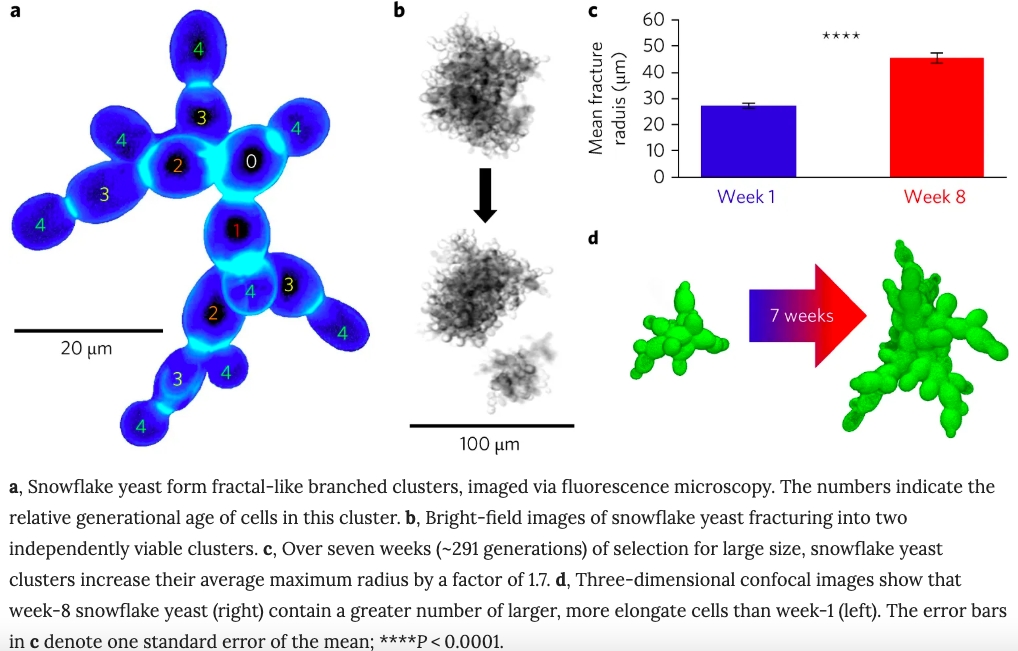
\includegraphics{https://pennykahn.github.io/biol501/Assignment_2/cluster.png}
\caption{}
\end{figure}

\section{Describe the Data}\label{describe-the-data}

The data I will use are from a plot showing the relationship between
number of cells and cluster size at two time points in the evolution
experiment. The response variable is number of cells in a cluster
(continuous, fixed), and the explanatory variables are cluster size
(continuous, fixed) and time point (categorical, fixed). Each individual
cluster has a measurement for size (radius, μm) and number of cells, as
well as a time point (either Week 1 or Week 8). All individuals were
measured from the same population which experienced daily selection
events for large size. Let's look at the data to get an idea of the
patterns.

First I'll read the data into a table called ``snowflake'' using the
here() function from the ``here'' package. This allows the code to work
for someone who has cloned the whole R project to a directory of their
choosing anywhere on their local system.

\begin{Shaded}
\begin{Highlighting}[]
\NormalTok{snowflake <-}\StringTok{ }\KeywordTok{read_csv}\NormalTok{(here}\OperatorTok{::}\KeywordTok{here}\NormalTok{(}\StringTok{"Assignment_2"}\NormalTok{, }\StringTok{"mod_attempt2.csv"}\NormalTok{))}
\end{Highlighting}
\end{Shaded}

\begin{verbatim}
## Parsed with column specification:
## cols(
##   radius = col_double(),
##   no_cells = col_double(),
##   week = col_character()
## )
\end{verbatim}

Let's take a look at the data using the datatable() function from the
``DT'' package. This prints a nice looking, interactive table.

\begin{Shaded}
\begin{Highlighting}[]
\NormalTok{snowflake}
\end{Highlighting}
\end{Shaded}

\begin{verbatim}
## # A tibble: 47 x 3
##    radius no_cells week  
##     <dbl>    <dbl> <chr> 
##  1   13.7       27 Week 1
##  2   21.7       69 Week 1
##  3   22.5      102 Week 1
##  4   22.6       88 Week 1
##  5   25.4      124 Week 1
##  6   26.4      175 Week 1
##  7   27.3      164 Week 1
##  8   28.0      147 Week 1
##  9   29.3      201 Week 1
## 10   29.8      195 Week 1
## # ... with 37 more rows
\end{verbatim}

We'll visualize it further with a scatter plot. The different colors
indicate time point.

\begin{Shaded}
\begin{Highlighting}[]
\NormalTok{plot <-}\StringTok{ }\NormalTok{snowflake }\OperatorTok
\StringTok{  }\KeywordTok{ggplot}\NormalTok{(}\KeywordTok{aes}\NormalTok{(}\DataTypeTok{x =}\NormalTok{ radius, }\DataTypeTok{y =}\NormalTok{ no_cells)) }\OperatorTok{+}
\StringTok{  }\KeywordTok{geom_point}\NormalTok{(}\KeywordTok{aes}\NormalTok{(}\DataTypeTok{color =}\NormalTok{ week)) }\OperatorTok{+}
\StringTok{  }\KeywordTok{labs}\NormalTok{(}\DataTypeTok{x =} \StringTok{"Cluster radius (μm)"}\NormalTok{, }\DataTypeTok{y =} \StringTok{"Number of cells"}\NormalTok{) }\OperatorTok{+}
\StringTok{  }\KeywordTok{theme_classic}\NormalTok{() }\OperatorTok{+}\StringTok{ }
\StringTok{  }\KeywordTok{theme}\NormalTok{(}\DataTypeTok{legend.title =} \KeywordTok{element_blank}\NormalTok{())}

\NormalTok{plot}
\end{Highlighting}
\end{Shaded}

\begin{verbatim}
## Warning in grid.Call(C_textBounds, as.graphicsAnnot(x$label), x$x,
## x$y, : conversion failure on 'Cluster radius (μm)' in 'mbcsToSbcs': dot
## substituted for <ce>
\end{verbatim}

\begin{verbatim}
## Warning in grid.Call(C_textBounds, as.graphicsAnnot(x$label), x$x,
## x$y, : conversion failure on 'Cluster radius (μm)' in 'mbcsToSbcs': dot
## substituted for <bc>
\end{verbatim}

\begin{verbatim}
## Warning in grid.Call(C_textBounds, as.graphicsAnnot(x$label), x$x,
## x$y, : conversion failure on 'Cluster radius (μm)' in 'mbcsToSbcs': dot
## substituted for <ce>
\end{verbatim}

\begin{verbatim}
## Warning in grid.Call(C_textBounds, as.graphicsAnnot(x$label), x$x,
## x$y, : conversion failure on 'Cluster radius (μm)' in 'mbcsToSbcs': dot
## substituted for <bc>
\end{verbatim}

\begin{verbatim}
## Warning in grid.Call(C_textBounds, as.graphicsAnnot(x$label), x$x,
## x$y, : conversion failure on 'Cluster radius (μm)' in 'mbcsToSbcs': dot
## substituted for <ce>
\end{verbatim}

\begin{verbatim}
## Warning in grid.Call(C_textBounds, as.graphicsAnnot(x$label), x$x,
## x$y, : conversion failure on 'Cluster radius (μm)' in 'mbcsToSbcs': dot
## substituted for <bc>
\end{verbatim}

\begin{verbatim}
## Warning in grid.Call(C_textBounds, as.graphicsAnnot(x$label), x$x,
## x$y, : conversion failure on 'Cluster radius (μm)' in 'mbcsToSbcs': dot
## substituted for <ce>
\end{verbatim}

\begin{verbatim}
## Warning in grid.Call(C_textBounds, as.graphicsAnnot(x$label), x$x,
## x$y, : conversion failure on 'Cluster radius (μm)' in 'mbcsToSbcs': dot
## substituted for <bc>
\end{verbatim}

\begin{verbatim}
## Warning in grid.Call(C_textBounds, as.graphicsAnnot(x$label), x$x,
## x$y, : conversion failure on 'Cluster radius (μm)' in 'mbcsToSbcs': dot
## substituted for <ce>
\end{verbatim}

\begin{verbatim}
## Warning in grid.Call(C_textBounds, as.graphicsAnnot(x$label), x$x,
## x$y, : conversion failure on 'Cluster radius (μm)' in 'mbcsToSbcs': dot
## substituted for <bc>
\end{verbatim}

\begin{verbatim}
## Warning in grid.Call(C_textBounds, as.graphicsAnnot(x$label), x$x,
## x$y, : conversion failure on 'Cluster radius (μm)' in 'mbcsToSbcs': dot
## substituted for <ce>
\end{verbatim}

\begin{verbatim}
## Warning in grid.Call(C_textBounds, as.graphicsAnnot(x$label), x$x,
## x$y, : conversion failure on 'Cluster radius (μm)' in 'mbcsToSbcs': dot
## substituted for <bc>
\end{verbatim}

\begin{verbatim}
## Warning in grid.Call(C_textBounds, as.graphicsAnnot(x$label), x$x,
## x$y, : conversion failure on 'Cluster radius (μm)' in 'mbcsToSbcs': dot
## substituted for <ce>
\end{verbatim}

\begin{verbatim}
## Warning in grid.Call(C_textBounds, as.graphicsAnnot(x$label), x$x,
## x$y, : conversion failure on 'Cluster radius (μm)' in 'mbcsToSbcs': dot
## substituted for <bc>
\end{verbatim}

\begin{verbatim}
## Warning in grid.Call.graphics(C_text, as.graphicsAnnot(x$label), x$x,
## x$y, : conversion failure on 'Cluster radius (μm)' in 'mbcsToSbcs': dot
## substituted for <ce>
\end{verbatim}

\begin{verbatim}
## Warning in grid.Call.graphics(C_text, as.graphicsAnnot(x$label), x$x,
## x$y, : conversion failure on 'Cluster radius (μm)' in 'mbcsToSbcs': dot
## substituted for <bc>
\end{verbatim}

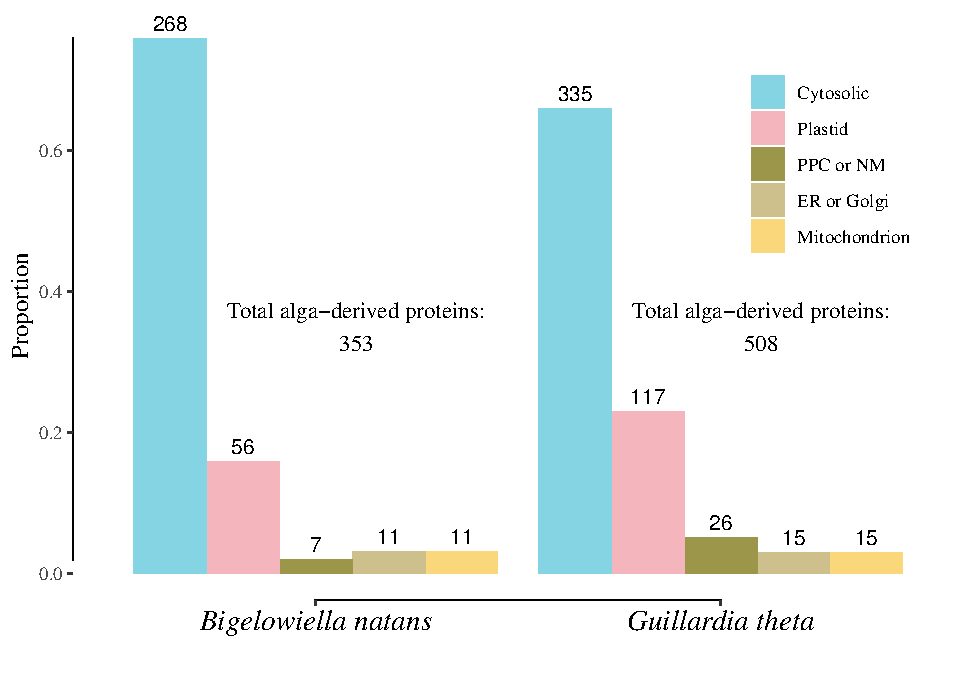
\includegraphics{Assignment2_forpdf_files/figure-latex/unnamed-chunk-4-1.pdf}

\subsubsection{Patterns}\label{patterns}

The first (perhaps obvious) pattern is that as cluster size increases,
so does the number of cells within a cluster. This makes sense because
cell division (and failure to separate mother and daughter) is how an
individual grows. A more meaningful pattern we can see from this graph
is that the distribution has shifted toward a larger cluster size from
week 1 to week 8, indicating that cluster size has in fact increased
over the course of the evolution experiment. Most importantly for the
context of the study, we see that for each cluster radius, the week 8
individuals have a lower number of cells than the week 1 individuals.
Remember, this is because the cells themselves are increasing in size
and aspect ratio.

\subsubsection{Parameters}\label{parameters}

A linear model fit to these data will provide us with estimates for
slope and intercepts of lines that fit the data depending on the
settings of the model.

\begin{itemize}
\tightlist
\item
  For a model with one explanatory and one response variable, we will
  receive an intercept and slope..
\item
  For a model with two explanatory variables we will receive an
  intercept and a slope for one line, and a value for the difference in
  intercept of another line. So we will get two parallel lines with
  different intercepts.
\item
  For a model with an interaction between two explanatory variables, we
  will receive an intercept and slope for one line, and values for the
  differences in the intercept and slope of the other line. So we will
  get two lines with different slopes and intercepts.
\item
  If we ask for a model with a second degree polynomial (y = b0 + b1X +
  b2X\^{}2), we will receive an estimate for the intercept (b0), the
  coefficient for the first term (b1), and the coefficient for the
  second term (b2). If we include an interaction with another
  explanatory variable, we will also receive all the estimates for
  differences in those three parameters for the second line.
\end{itemize}

\subsubsection{Hypotheses}\label{hypotheses}

\begin{enumerate}
\def\labelenumi{\arabic{enumi}.}
\tightlist
\item
  There is a positive linear relationship between size and cell number
  in general.
\item
  The group means at each time point are actually different from one
  another (there should be a different intercept for each time point).
\item
  There is an interaction between time point and cluster size (there
  should be a different slope and intercept for each time point).
\item
  Adding a second degree polynomial factor will fit the data better than
  a straight line.
\end{enumerate}

\section{Fit a Linear Model}\label{fit-a-linear-model}

I don't think this is necessary for the assignment, but I'm going to fit
a few models (instead of just one) with increasing complexity to show
how different models fit the data. I think it's useful to show how each
added term affects the model, and discuss the changing implications for
interpretation of the data.

\subsection{The simplest linear model}\label{the-simplest-linear-model}

This first model will be the simplest. It will look at the overall
relationship between cluster size (explanatory) and number of cells in a
cluster (response). The output we get from this model will give us
estimates for slope and intercept of one line (y = b0 + b1*X) that fits
the entire dataset.

\begin{Shaded}
\begin{Highlighting}[]
\NormalTok{mod_}\DecValTok{1}\NormalTok{ <-}\StringTok{ }\KeywordTok{lm}\NormalTok{(no_cells }\OperatorTok{~}\StringTok{ }\NormalTok{radius, }\DataTypeTok{data =}\NormalTok{ snowflake)}
\KeywordTok{summary}\NormalTok{(mod_}\DecValTok{1}\NormalTok{)}
\end{Highlighting}
\end{Shaded}

\begin{verbatim}
## 
## Call:
## lm(formula = no_cells ~ radius, data = snowflake)
## 
## Residuals:
##    Min     1Q Median     3Q    Max 
## -96.25 -57.46 -39.16  43.86 233.20 
## 
## Coefficients:
##             Estimate Std. Error t value Pr(>|t|)    
## (Intercept) -123.364     59.832  -2.062    0.045 *  
## radius         9.599      1.765   5.439 2.11e-06 ***
## ---
## Signif. codes:  0 '***' 0.001 '**' 0.01 '*' 0.05 '.' 0.1 ' ' 1
## 
## Residual standard error: 82.55 on 45 degrees of freedom
## Multiple R-squared:  0.3966, Adjusted R-squared:  0.3832 
## F-statistic: 29.58 on 1 and 45 DF,  p-value: 2.106e-06
\end{verbatim}

The (Intercept) estimate gives the intercept of the line, but it's not
very biologically relevant as it is not possible to have a cluster size
of 0 μm. In fact a single yeast cell has a radius of about 2.5 to 5 μm.
This value determines the line's position on the y-axis. The model picks
a position that will minimize residuals. In this case, for the purpose
of the model, when cluster radius is 0 the number of cells is -123.364.

The ``radius'' estimate gives us the slope of the line. In this simplest
model, with every 1 μm increase in cluster radius, there is a cell
number increase of 9.599. The sign of the value demonstrates a positive
relationship between cluster size and number of cells in a cluster,
which again should be obvious.

\begin{center}\rule{0.5\linewidth}{\linethickness}\end{center}

I'll perform an ANOVA to test our first model against a null hypothesis
of no relationship.

\begin{Shaded}
\begin{Highlighting}[]
\KeywordTok{anova}\NormalTok{(mod_}\DecValTok{1}\NormalTok{)}
\end{Highlighting}
\end{Shaded}

\begin{verbatim}
## Analysis of Variance Table
## 
## Response: no_cells
##           Df Sum Sq Mean Sq F value    Pr(>F)    
## radius     1 201593  201593  29.583 2.106e-06 ***
## Residuals 45 306654    6815                      
## ---
## Signif. codes:  0 '***' 0.001 '**' 0.01 '*' 0.05 '.' 0.1 ' ' 1
\end{verbatim}

This ANOVA provides us with a p-value for comparing the model we have
created (mod1) with a null model which assumes no positive or negative
relationship between the variables. The null model tries to fit the data
to the average response. The ANOVA yields a p-value of 2.106e-06, so
based on p-value alone our simple model fits the data better than the
null model. We can conclude there is a relationship between cluster size
and number of cells.

\begin{center}\rule{0.5\linewidth}{\linethickness}\end{center}

Now let's visualize the fit of the model to the data. I'll use the
geom\_abline() function to easily specify intercept and slope, which I
have taken from the model output.

\begin{Shaded}
\begin{Highlighting}[]
\NormalTok{plot1 <-}\StringTok{ }\NormalTok{plot }\OperatorTok{+}\StringTok{ }
\StringTok{  }\KeywordTok{geom_abline}\NormalTok{(}\DataTypeTok{intercept =} \OperatorTok{-}\FloatTok{123.364}\NormalTok{, }\DataTypeTok{slope =} \FloatTok{9.599}\NormalTok{)}

\NormalTok{plot1}
\end{Highlighting}
\end{Shaded}

\begin{verbatim}
## Warning in grid.Call(C_textBounds, as.graphicsAnnot(x$label), x$x,
## x$y, : conversion failure on 'Cluster radius (μm)' in 'mbcsToSbcs': dot
## substituted for <ce>
\end{verbatim}

\begin{verbatim}
## Warning in grid.Call(C_textBounds, as.graphicsAnnot(x$label), x$x,
## x$y, : conversion failure on 'Cluster radius (μm)' in 'mbcsToSbcs': dot
## substituted for <bc>
\end{verbatim}

\begin{verbatim}
## Warning in grid.Call(C_textBounds, as.graphicsAnnot(x$label), x$x,
## x$y, : conversion failure on 'Cluster radius (μm)' in 'mbcsToSbcs': dot
## substituted for <ce>
\end{verbatim}

\begin{verbatim}
## Warning in grid.Call(C_textBounds, as.graphicsAnnot(x$label), x$x,
## x$y, : conversion failure on 'Cluster radius (μm)' in 'mbcsToSbcs': dot
## substituted for <bc>
\end{verbatim}

\begin{verbatim}
## Warning in grid.Call(C_textBounds, as.graphicsAnnot(x$label), x$x,
## x$y, : conversion failure on 'Cluster radius (μm)' in 'mbcsToSbcs': dot
## substituted for <ce>
\end{verbatim}

\begin{verbatim}
## Warning in grid.Call(C_textBounds, as.graphicsAnnot(x$label), x$x,
## x$y, : conversion failure on 'Cluster radius (μm)' in 'mbcsToSbcs': dot
## substituted for <bc>
\end{verbatim}

\begin{verbatim}
## Warning in grid.Call(C_textBounds, as.graphicsAnnot(x$label), x$x,
## x$y, : conversion failure on 'Cluster radius (μm)' in 'mbcsToSbcs': dot
## substituted for <ce>
\end{verbatim}

\begin{verbatim}
## Warning in grid.Call(C_textBounds, as.graphicsAnnot(x$label), x$x,
## x$y, : conversion failure on 'Cluster radius (μm)' in 'mbcsToSbcs': dot
## substituted for <bc>
\end{verbatim}

\begin{verbatim}
## Warning in grid.Call(C_textBounds, as.graphicsAnnot(x$label), x$x,
## x$y, : conversion failure on 'Cluster radius (μm)' in 'mbcsToSbcs': dot
## substituted for <ce>
\end{verbatim}

\begin{verbatim}
## Warning in grid.Call(C_textBounds, as.graphicsAnnot(x$label), x$x,
## x$y, : conversion failure on 'Cluster radius (μm)' in 'mbcsToSbcs': dot
## substituted for <bc>
\end{verbatim}

\begin{verbatim}
## Warning in grid.Call(C_textBounds, as.graphicsAnnot(x$label), x$x,
## x$y, : conversion failure on 'Cluster radius (μm)' in 'mbcsToSbcs': dot
## substituted for <ce>
\end{verbatim}

\begin{verbatim}
## Warning in grid.Call(C_textBounds, as.graphicsAnnot(x$label), x$x,
## x$y, : conversion failure on 'Cluster radius (μm)' in 'mbcsToSbcs': dot
## substituted for <bc>
\end{verbatim}

\begin{verbatim}
## Warning in grid.Call(C_textBounds, as.graphicsAnnot(x$label), x$x,
## x$y, : conversion failure on 'Cluster radius (μm)' in 'mbcsToSbcs': dot
## substituted for <ce>
\end{verbatim}

\begin{verbatim}
## Warning in grid.Call(C_textBounds, as.graphicsAnnot(x$label), x$x,
## x$y, : conversion failure on 'Cluster radius (μm)' in 'mbcsToSbcs': dot
## substituted for <bc>
\end{verbatim}

\begin{verbatim}
## Warning in grid.Call.graphics(C_text, as.graphicsAnnot(x$label), x$x,
## x$y, : conversion failure on 'Cluster radius (μm)' in 'mbcsToSbcs': dot
## substituted for <ce>
\end{verbatim}

\begin{verbatim}
## Warning in grid.Call.graphics(C_text, as.graphicsAnnot(x$label), x$x,
## x$y, : conversion failure on 'Cluster radius (μm)' in 'mbcsToSbcs': dot
## substituted for <bc>
\end{verbatim}

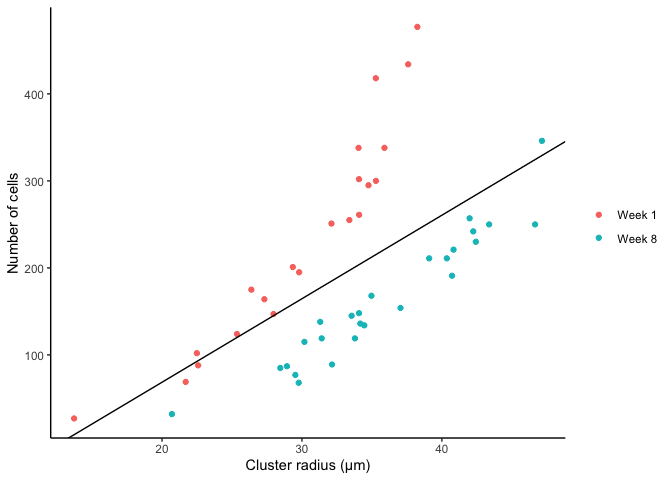
\includegraphics{Assignment2_forpdf_files/figure-latex/unnamed-chunk-7-1.pdf}

This graph simply shows a positive relationship. Number of cells in a
cluster increases with cluster radius. We can see the line doesn't fit
the data perfectly. It mostly goes down the middle of two groups:
samples from week 1 and week 8. I think it's easy to see that there
should be separate lines for each time point.

\subsection{Adding time point
variable}\label{adding-time-point-variable}

Now I'll add in the categorical explanatory variable of time point. We
should still see a positive relationship for both groups within the
explanatory variable ``week'', but they will have different intercepts,
and therefore different positions in graphical space.

\begin{Shaded}
\begin{Highlighting}[]
\NormalTok{mod_}\DecValTok{2}\NormalTok{ <-}\StringTok{ }\KeywordTok{lm}\NormalTok{(no_cells }\OperatorTok{~}\StringTok{ }\NormalTok{radius }\OperatorTok{+}\StringTok{ }\NormalTok{week, }\DataTypeTok{data =}\NormalTok{ snowflake)}
\KeywordTok{summary}\NormalTok{(mod_}\DecValTok{2}\NormalTok{)}
\end{Highlighting}
\end{Shaded}

\begin{verbatim}
## 
## Call:
## lm(formula = no_cells ~ radius + week, data = snowflake)
## 
## Residuals:
##    Min     1Q Median     3Q    Max 
## -68.16 -26.56  -9.20  18.48 124.06 
## 
## Coefficients:
##              Estimate Std. Error t value Pr(>|t|)    
## (Intercept) -192.6535    30.7060  -6.274 1.33e-07 ***
## radius        14.2644     0.9757  14.620  < 2e-16 ***
## weekWeek 8  -154.7785    13.3895 -11.560 6.36e-15 ***
## ---
## Signif. codes:  0 '***' 0.001 '**' 0.01 '*' 0.05 '.' 0.1 ' ' 1
## 
## Residual standard error: 41.55 on 44 degrees of freedom
## Multiple R-squared:  0.8505, Adjusted R-squared:  0.8437 
## F-statistic: 125.2 on 2 and 44 DF,  p-value: < 2.2e-16
\end{verbatim}

Now we have three coefficient estimates. In the order given in the
output, we have the intercept for week 1, the slope for both weeks, and
a difference of intercept for week 8. We can use the values from this
output to make two regression equations - one for each week. The
intercepts for the lines are -192.6535 for week 1 and (-192.6535 -
154.7785) or -347.432 for week 8. This estimates that for a given
cluster radius there will be \textasciitilde{}155 cells fewer in week 8
than week 1.

We see that the slope has increased from the first model (14.2644
\textgreater{} 9.599). Mod2 predicts that for a 1 μm increase in cluster
radius, there is a cell number increase of 14.2644. This increase in
slope is because the relationship in the first model was being obscured
by the difference in distribution along the x-axis. Also, the adjusted
r-squared value has increased from the first to the second model (0.8437
\textgreater{} 0.3832) indicating a tighter fit of the data to the
lines.

\begin{center}\rule{0.5\linewidth}{\linethickness}\end{center}

I'll test if the second model which includes the explanatory variable of
``week'' is significantly different from the first using an ANOVA again.

\begin{Shaded}
\begin{Highlighting}[]
\KeywordTok{anova}\NormalTok{(mod_}\DecValTok{2}\NormalTok{, mod_}\DecValTok{1}\NormalTok{)}
\end{Highlighting}
\end{Shaded}

\begin{verbatim}
## Analysis of Variance Table
## 
## Model 1: no_cells ~ radius + week
## Model 2: no_cells ~ radius
##   Res.Df    RSS Df Sum of Sq      F    Pr(>F)    
## 1     44  75962                                  
## 2     45 306654 -1   -230692 133.63 6.358e-15 ***
## ---
## Signif. codes:  0 '***' 0.001 '**' 0.01 '*' 0.05 '.' 0.1 ' ' 1
\end{verbatim}

This ANOVA is comparing a model that includes time point as an
explanatory variable as well as cluster size to the first model which
only includes cluster size. Since we have a significant p-value we can
conclude that there is a difference in group mean between the two weeks,
and the model we choose should reflect that. In other words, using week
and cluster size to predict number of cells in a cluster will yield a
more accurate prediction than using cluster size alone.

\begin{center}\rule{0.5\linewidth}{\linethickness}\end{center}

We'll visualize the model fit to the data using the same method as
before. I'm adding the first and third coefficient estimates for for the
intercept of the second line.

\begin{Shaded}
\begin{Highlighting}[]
\NormalTok{plot2 <-}\StringTok{ }\NormalTok{plot }\OperatorTok{+}
\StringTok{  }\KeywordTok{geom_abline}\NormalTok{(}\DataTypeTok{intercept =} \OperatorTok{-}\FloatTok{192.6535}\NormalTok{, }\DataTypeTok{slope =} \FloatTok{14.2644}\NormalTok{) }\OperatorTok{+}
\StringTok{  }\KeywordTok{geom_abline}\NormalTok{(}\DataTypeTok{intercept =}\NormalTok{ (}\OperatorTok{-}\FloatTok{192.6535} \OperatorTok{-}\StringTok{ }\FloatTok{154.7785}\NormalTok{), }\DataTypeTok{slope =} \FloatTok{14.2644}\NormalTok{)}

\NormalTok{plot2}
\end{Highlighting}
\end{Shaded}

\begin{verbatim}
## Warning in grid.Call(C_textBounds, as.graphicsAnnot(x$label), x$x,
## x$y, : conversion failure on 'Cluster radius (μm)' in 'mbcsToSbcs': dot
## substituted for <ce>
\end{verbatim}

\begin{verbatim}
## Warning in grid.Call(C_textBounds, as.graphicsAnnot(x$label), x$x,
## x$y, : conversion failure on 'Cluster radius (μm)' in 'mbcsToSbcs': dot
## substituted for <bc>
\end{verbatim}

\begin{verbatim}
## Warning in grid.Call(C_textBounds, as.graphicsAnnot(x$label), x$x,
## x$y, : conversion failure on 'Cluster radius (μm)' in 'mbcsToSbcs': dot
## substituted for <ce>
\end{verbatim}

\begin{verbatim}
## Warning in grid.Call(C_textBounds, as.graphicsAnnot(x$label), x$x,
## x$y, : conversion failure on 'Cluster radius (μm)' in 'mbcsToSbcs': dot
## substituted for <bc>
\end{verbatim}

\begin{verbatim}
## Warning in grid.Call(C_textBounds, as.graphicsAnnot(x$label), x$x,
## x$y, : conversion failure on 'Cluster radius (μm)' in 'mbcsToSbcs': dot
## substituted for <ce>
\end{verbatim}

\begin{verbatim}
## Warning in grid.Call(C_textBounds, as.graphicsAnnot(x$label), x$x,
## x$y, : conversion failure on 'Cluster radius (μm)' in 'mbcsToSbcs': dot
## substituted for <bc>
\end{verbatim}

\begin{verbatim}
## Warning in grid.Call(C_textBounds, as.graphicsAnnot(x$label), x$x,
## x$y, : conversion failure on 'Cluster radius (μm)' in 'mbcsToSbcs': dot
## substituted for <ce>
\end{verbatim}

\begin{verbatim}
## Warning in grid.Call(C_textBounds, as.graphicsAnnot(x$label), x$x,
## x$y, : conversion failure on 'Cluster radius (μm)' in 'mbcsToSbcs': dot
## substituted for <bc>
\end{verbatim}

\begin{verbatim}
## Warning in grid.Call(C_textBounds, as.graphicsAnnot(x$label), x$x,
## x$y, : conversion failure on 'Cluster radius (μm)' in 'mbcsToSbcs': dot
## substituted for <ce>
\end{verbatim}

\begin{verbatim}
## Warning in grid.Call(C_textBounds, as.graphicsAnnot(x$label), x$x,
## x$y, : conversion failure on 'Cluster radius (μm)' in 'mbcsToSbcs': dot
## substituted for <bc>
\end{verbatim}

\begin{verbatim}
## Warning in grid.Call(C_textBounds, as.graphicsAnnot(x$label), x$x,
## x$y, : conversion failure on 'Cluster radius (μm)' in 'mbcsToSbcs': dot
## substituted for <ce>
\end{verbatim}

\begin{verbatim}
## Warning in grid.Call(C_textBounds, as.graphicsAnnot(x$label), x$x,
## x$y, : conversion failure on 'Cluster radius (μm)' in 'mbcsToSbcs': dot
## substituted for <bc>
\end{verbatim}

\begin{verbatim}
## Warning in grid.Call(C_textBounds, as.graphicsAnnot(x$label), x$x,
## x$y, : conversion failure on 'Cluster radius (μm)' in 'mbcsToSbcs': dot
## substituted for <ce>
\end{verbatim}

\begin{verbatim}
## Warning in grid.Call(C_textBounds, as.graphicsAnnot(x$label), x$x,
## x$y, : conversion failure on 'Cluster radius (μm)' in 'mbcsToSbcs': dot
## substituted for <bc>
\end{verbatim}

\begin{verbatim}
## Warning in grid.Call.graphics(C_text, as.graphicsAnnot(x$label), x$x,
## x$y, : conversion failure on 'Cluster radius (μm)' in 'mbcsToSbcs': dot
## substituted for <ce>
\end{verbatim}

\begin{verbatim}
## Warning in grid.Call.graphics(C_text, as.graphicsAnnot(x$label), x$x,
## x$y, : conversion failure on 'Cluster radius (μm)' in 'mbcsToSbcs': dot
## substituted for <bc>
\end{verbatim}

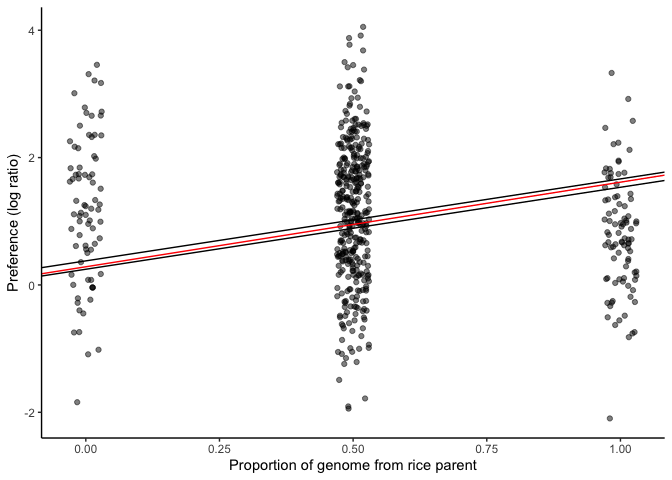
\includegraphics{Assignment2_forpdf_files/figure-latex/unnamed-chunk-10-1.pdf}

We can still see the positive relationship between cluster size and
number of cells, but we can see that over time (from week 1 to week 8)
the distribution has shifted right on the x-axis and down on the y-axis,
that is, the cluster size has increased overall with a fewer number of
cells at each size.

These lines appear to fit the data better than a single line for both
weeks, but it might be better to have different slopes for each week, so
I'll add an interaction term between week and cluster size.

\subsection{Interaction component}\label{interaction-component}

I'll add an interaction between week and radius by putting an asterisk
between them instead of a plus sign.

\begin{Shaded}
\begin{Highlighting}[]
\NormalTok{mod_}\DecValTok{3}\NormalTok{ <-}\StringTok{ }\KeywordTok{lm}\NormalTok{(no_cells }\OperatorTok{~}\StringTok{ }\NormalTok{radius }\OperatorTok{*}\StringTok{ }\NormalTok{week, }\DataTypeTok{data =}\NormalTok{ snowflake)}
\KeywordTok{summary}\NormalTok{(mod_}\DecValTok{3}\NormalTok{)}
\end{Highlighting}
\end{Shaded}

\begin{verbatim}
## 
## Call:
## lm(formula = no_cells ~ radius * week, data = snowflake)
## 
## Residuals:
##     Min      1Q  Median      3Q     Max 
## -50.736 -22.746  -5.028   9.483  90.868 
## 
## Coefficients:
##                   Estimate Std. Error t value Pr(>|t|)    
## (Intercept)       -314.641     38.029  -8.274 1.95e-10 ***
## radius              18.322      1.239  14.787  < 2e-16 ***
## weekWeek 8          80.791     55.040   1.468    0.149    
## radius:weekWeek 8   -7.235      1.655  -4.373 7.66e-05 ***
## ---
## Signif. codes:  0 '***' 0.001 '**' 0.01 '*' 0.05 '.' 0.1 ' ' 1
## 
## Residual standard error: 34.97 on 43 degrees of freedom
## Multiple R-squared:  0.8965, Adjusted R-squared:  0.8893 
## F-statistic: 124.2 on 3 and 43 DF,  p-value: < 2.2e-16
\end{verbatim}

In the output of the interaction model we have four coefficient
estimates. In order they are: the intercept of the week 1 line, the
slope of the week 1 line, the difference in intercept of the week 8
line, and the difference in slope of the week 8 line.

Since the slope is different for each line, the difference in intercept
is less biologically interpretable on its own. The models estimate that
at a cluster size of 0 μm, the number of cells will be -314.641 in week
1 (meaningless) and (-314.641 + 80.791) or -233.85 in week 8 (also
meaningless). Since the slopes are different, this difference in cell
number between the two weeks at a given cluster size will change as a
function of the slopes.

The interpretation of the slopes is more biologically relevant. In week
1, with every cluster size increase of 1 μm, there will be 18.322 more
cells. In week 8, with an increase of 1 μm there will be (18.322 -
7.235) or 11.087 more cells. Fewer cells are needed to generate the same
size increase.

Again we can see that the R-squared value has increased from mod2
(0.8437) to mod3 (0.8893).

\begin{center}\rule{0.5\linewidth}{\linethickness}\end{center}

Now we'll use an ANOVA to test if week and cluster size interact
significantly.

\begin{Shaded}
\begin{Highlighting}[]
\KeywordTok{anova}\NormalTok{(mod_}\DecValTok{3}\NormalTok{, mod_}\DecValTok{2}\NormalTok{)}
\end{Highlighting}
\end{Shaded}

\begin{verbatim}
## Analysis of Variance Table
## 
## Model 1: no_cells ~ radius * week
## Model 2: no_cells ~ radius + week
##   Res.Df   RSS Df Sum of Sq      F    Pr(>F)    
## 1     43 52582                                  
## 2     44 75962 -1    -23380 19.119 7.659e-05 ***
## ---
## Signif. codes:  0 '***' 0.001 '**' 0.01 '*' 0.05 '.' 0.1 ' ' 1
\end{verbatim}

This significant p-value indicates that there is an interaction with
week and there should be different slopes for each line. The trends for
how clusters grow at each time point are significantly different. We can
more accurately predict number of cells per cluster by using different
slopes and intercepts for each week instead of just having two parallel
lines.

\begin{center}\rule{0.5\linewidth}{\linethickness}\end{center}

To add the lines to this plot, I'm using geom\_abline() again, but now I
also add the difference between slopes to the second line.

\begin{Shaded}
\begin{Highlighting}[]
\NormalTok{plot3 <-}\StringTok{ }\NormalTok{plot }\OperatorTok{+}\StringTok{ }
\StringTok{  }\KeywordTok{geom_abline}\NormalTok{(}\DataTypeTok{intercept =} \OperatorTok{-}\FloatTok{314.641}\NormalTok{, }\DataTypeTok{slope =} \FloatTok{18.322}\NormalTok{) }\OperatorTok{+}
\StringTok{  }\KeywordTok{geom_abline}\NormalTok{(}\DataTypeTok{intercept =}\NormalTok{ (}\OperatorTok{-}\FloatTok{314.641} \OperatorTok{+}\StringTok{ }\FloatTok{80.791}\NormalTok{), }\DataTypeTok{slope =}\NormalTok{ (}\FloatTok{18.322} \OperatorTok{-}\StringTok{ }\FloatTok{7.235}\NormalTok{))}

\NormalTok{plot3}
\end{Highlighting}
\end{Shaded}

\begin{verbatim}
## Warning in grid.Call(C_textBounds, as.graphicsAnnot(x$label), x$x,
## x$y, : conversion failure on 'Cluster radius (μm)' in 'mbcsToSbcs': dot
## substituted for <ce>
\end{verbatim}

\begin{verbatim}
## Warning in grid.Call(C_textBounds, as.graphicsAnnot(x$label), x$x,
## x$y, : conversion failure on 'Cluster radius (μm)' in 'mbcsToSbcs': dot
## substituted for <bc>
\end{verbatim}

\begin{verbatim}
## Warning in grid.Call(C_textBounds, as.graphicsAnnot(x$label), x$x,
## x$y, : conversion failure on 'Cluster radius (μm)' in 'mbcsToSbcs': dot
## substituted for <ce>
\end{verbatim}

\begin{verbatim}
## Warning in grid.Call(C_textBounds, as.graphicsAnnot(x$label), x$x,
## x$y, : conversion failure on 'Cluster radius (μm)' in 'mbcsToSbcs': dot
## substituted for <bc>
\end{verbatim}

\begin{verbatim}
## Warning in grid.Call(C_textBounds, as.graphicsAnnot(x$label), x$x,
## x$y, : conversion failure on 'Cluster radius (μm)' in 'mbcsToSbcs': dot
## substituted for <ce>
\end{verbatim}

\begin{verbatim}
## Warning in grid.Call(C_textBounds, as.graphicsAnnot(x$label), x$x,
## x$y, : conversion failure on 'Cluster radius (μm)' in 'mbcsToSbcs': dot
## substituted for <bc>
\end{verbatim}

\begin{verbatim}
## Warning in grid.Call(C_textBounds, as.graphicsAnnot(x$label), x$x,
## x$y, : conversion failure on 'Cluster radius (μm)' in 'mbcsToSbcs': dot
## substituted for <ce>
\end{verbatim}

\begin{verbatim}
## Warning in grid.Call(C_textBounds, as.graphicsAnnot(x$label), x$x,
## x$y, : conversion failure on 'Cluster radius (μm)' in 'mbcsToSbcs': dot
## substituted for <bc>
\end{verbatim}

\begin{verbatim}
## Warning in grid.Call(C_textBounds, as.graphicsAnnot(x$label), x$x,
## x$y, : conversion failure on 'Cluster radius (μm)' in 'mbcsToSbcs': dot
## substituted for <ce>
\end{verbatim}

\begin{verbatim}
## Warning in grid.Call(C_textBounds, as.graphicsAnnot(x$label), x$x,
## x$y, : conversion failure on 'Cluster radius (μm)' in 'mbcsToSbcs': dot
## substituted for <bc>
\end{verbatim}

\begin{verbatim}
## Warning in grid.Call(C_textBounds, as.graphicsAnnot(x$label), x$x,
## x$y, : conversion failure on 'Cluster radius (μm)' in 'mbcsToSbcs': dot
## substituted for <ce>
\end{verbatim}

\begin{verbatim}
## Warning in grid.Call(C_textBounds, as.graphicsAnnot(x$label), x$x,
## x$y, : conversion failure on 'Cluster radius (μm)' in 'mbcsToSbcs': dot
## substituted for <bc>
\end{verbatim}

\begin{verbatim}
## Warning in grid.Call(C_textBounds, as.graphicsAnnot(x$label), x$x,
## x$y, : conversion failure on 'Cluster radius (μm)' in 'mbcsToSbcs': dot
## substituted for <ce>
\end{verbatim}

\begin{verbatim}
## Warning in grid.Call(C_textBounds, as.graphicsAnnot(x$label), x$x,
## x$y, : conversion failure on 'Cluster radius (μm)' in 'mbcsToSbcs': dot
## substituted for <bc>
\end{verbatim}

\begin{verbatim}
## Warning in grid.Call.graphics(C_text, as.graphicsAnnot(x$label), x$x,
## x$y, : conversion failure on 'Cluster radius (μm)' in 'mbcsToSbcs': dot
## substituted for <ce>
\end{verbatim}

\begin{verbatim}
## Warning in grid.Call.graphics(C_text, as.graphicsAnnot(x$label), x$x,
## x$y, : conversion failure on 'Cluster radius (μm)' in 'mbcsToSbcs': dot
## substituted for <bc>
\end{verbatim}

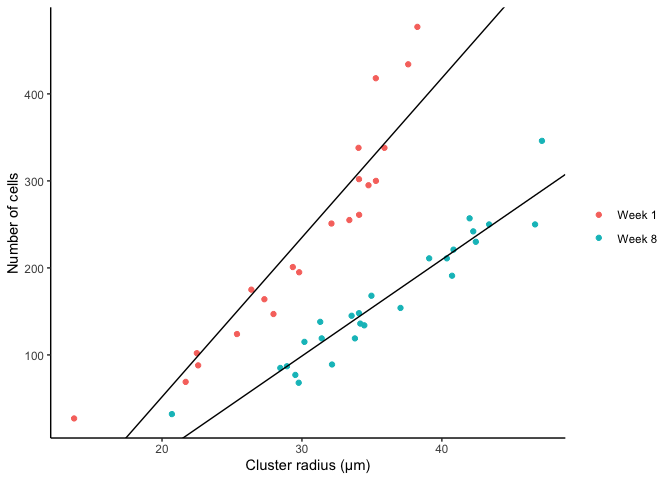
\includegraphics{Assignment2_forpdf_files/figure-latex/unnamed-chunk-13-1.pdf}

We can observe the larger slope for week 1 through its steeper incline.
More cells are needed to produce the same size increase in week 1 than
in week 8. In week 8 cells are larger, so each addition of a cell will
provide more volume to the cluster than a tiny week 1 cell will.

\subsection{Polynomial factor}\label{polynomial-factor}

The data don't look very linear because the nature of cluster growth is
not linear. With each generation time (i.e.~every time a yeast cell
divides) every cell within the cluster gets a new daughter (the ones on
the inside and the ones on the outside). The larger a cluster grows, the
less effect one division cycle has on the size of the overall cluster,
which we can see especially well in the week 1 sample. Even as number of
cells increases from \textasciitilde{}250 to almost 500, there is little
increase in cluster size. So I think a model that includes a second
degree polynomial will fit the data better than straight lines.

\begin{Shaded}
\begin{Highlighting}[]
\NormalTok{mod_}\DecValTok{4}\NormalTok{ <-}\StringTok{ }\KeywordTok{lm}\NormalTok{(no_cells }\OperatorTok{~}\StringTok{ }\KeywordTok{poly}\NormalTok{(radius, }\DecValTok{2}\NormalTok{, }\DataTypeTok{raw =} \OtherTok{TRUE}\NormalTok{) }\OperatorTok{*}\StringTok{ }\NormalTok{week, }\DataTypeTok{data =}\NormalTok{ snowflake)}
\KeywordTok{summary}\NormalTok{(mod_}\DecValTok{4}\NormalTok{)}
\end{Highlighting}
\end{Shaded}

\begin{verbatim}
## 
## Call:
## lm(formula = no_cells ~ poly(radius, 2, raw = TRUE) * week, data = snowflake)
## 
## Residuals:
##    Min     1Q Median     3Q    Max 
## -49.01 -15.49   0.25  14.75  74.16 
## 
## Coefficients:
##                                          Estimate Std. Error t value
## (Intercept)                              197.9767    93.6365   2.114
## poly(radius, 2, raw = TRUE)1             -21.4283     6.9801  -3.070
## poly(radius, 2, raw = TRUE)2               0.7246     0.1261   5.746
## weekWeek 8                              -210.8983   160.9878  -1.310
## poly(radius, 2, raw = TRUE)1:weekWeek 8   19.6616    10.2200   1.924
## poly(radius, 2, raw = TRUE)2:weekWeek 8   -0.5435     0.1638  -3.317
##                                         Pr(>|t|)    
## (Intercept)                              0.04061 *  
## poly(radius, 2, raw = TRUE)1             0.00379 ** 
## poly(radius, 2, raw = TRUE)2            9.95e-07 ***
## weekWeek 8                               0.19748    
## poly(radius, 2, raw = TRUE)1:weekWeek 8  0.06134 .  
## poly(radius, 2, raw = TRUE)2:weekWeek 8  0.00191 ** 
## ---
## Signif. codes:  0 '***' 0.001 '**' 0.01 '*' 0.05 '.' 0.1 ' ' 1
## 
## Residual standard error: 26.13 on 41 degrees of freedom
## Multiple R-squared:  0.9449, Adjusted R-squared:  0.9382 
## F-statistic: 140.7 on 5 and 41 DF,  p-value: < 2.2e-16
\end{verbatim}

There's a lot of coefficient estimates in this one. Basically, there's
an estimate for b0, b1, and b2 for week 1 as well as the differences in
all those coefficients for the week 8 function. And those get plugged
into the quadratic function y = b0 + b1X + b2X\^{}2. I was having a hard
time interpreting the biological significance of polynomial parameter
estimates, but then I found this from Stimson, J.A., Carmines, E.G.,
Zeller, R.A. 1978. Interpreting Polynomial Regression.
\emph{Sociological Methods \& Research} 6, 515-524:

\begin{quote}
\emph{``What meaning can be attributed to the individual coefficients in
polynomial regression equations? Unfortunately, these coefficients
cannot be easily or readily interpreted, partly because they are
noncomparable. For example, by definition Bl and B2 measure the change
in Y associated with each unit change of X or X2, respectively,
controlling for the effects of the other.''}
\end{quote}

So I'm going to leave it at that. Just as a note, I'll mention that the
positive sign of the coefficient b2 means the graph is convex
(u-shaped). b2 also tells us about the steepness of the curvature. Since
b2 is larger in the week 1 function, the u shape will be steeper than in
week 8. Apparently b1 gives the rate of change when x is equal to zero.

\begin{center}\rule{0.5\linewidth}{\linethickness}\end{center}

Anyway\ldots{} let's move onto the ANOVA to test if this quadratic
function is a better model than straight lines.

\begin{Shaded}
\begin{Highlighting}[]
\KeywordTok{anova}\NormalTok{(mod_}\DecValTok{4}\NormalTok{, mod_}\DecValTok{3}\NormalTok{)}
\end{Highlighting}
\end{Shaded}

\begin{verbatim}
## Analysis of Variance Table
## 
## Model 1: no_cells ~ poly(radius, 2, raw = TRUE) * week
## Model 2: no_cells ~ radius * week
##   Res.Df   RSS Df Sum of Sq      F    Pr(>F)    
## 1     41 27994                                  
## 2     43 52582 -2    -24588 18.006 2.441e-06 ***
## ---
## Signif. codes:  0 '***' 0.001 '**' 0.01 '*' 0.05 '.' 0.1 ' ' 1
\end{verbatim}

Indeed, the p-value is significant. The polynomial model fits the data
data significantly better than one that produces linear equations.

\begin{center}\rule{0.5\linewidth}{\linethickness}\end{center}

Here I'm writing the two functions, one for each week, using the
coefficient estimates from the summary of mod4. I'll use those set
functions to graph their lines in ggplot. I'm limiting the y-axis to 500
because otherwise it shows the line up to y = 800 even though there are
no data associated with that range.

\begin{Shaded}
\begin{Highlighting}[]
\NormalTok{poly1 <-}\StringTok{ }\ControlFlowTok{function}\NormalTok{(x) }\FloatTok{197.9767} \OperatorTok{-}\StringTok{ }\FloatTok{21.4283} \OperatorTok{*}\StringTok{ }\NormalTok{x }\OperatorTok{+}\StringTok{ }\FloatTok{0.7246} \OperatorTok{*}\StringTok{ }\NormalTok{x}\OperatorTok{^}\DecValTok{2}
\NormalTok{poly2 <-}\StringTok{ }\ControlFlowTok{function}\NormalTok{(x) (}\FloatTok{197.9767} \OperatorTok{-}\StringTok{ }\FloatTok{210.8983}\NormalTok{) }\OperatorTok{+}\StringTok{ }\NormalTok{(}\OperatorTok{-}\FloatTok{21.4283} \OperatorTok{+}\StringTok{ }\FloatTok{19.6616}\NormalTok{) }\OperatorTok{*}\StringTok{ }\NormalTok{x }\OperatorTok{+}\StringTok{ }\NormalTok{(}\FloatTok{0.7246} \OperatorTok{-}\StringTok{ }\FloatTok{0.5435}\NormalTok{) }\OperatorTok{*}\StringTok{ }\NormalTok{x}\OperatorTok{^}\DecValTok{2}
\end{Highlighting}
\end{Shaded}

\begin{Shaded}
\begin{Highlighting}[]
\NormalTok{plot4 <-}\StringTok{ }\NormalTok{plot }\OperatorTok{+}
\StringTok{  }\KeywordTok{stat_function}\NormalTok{(}\DataTypeTok{method =}\NormalTok{ lm, }\DataTypeTok{fun =}\NormalTok{ poly1) }\OperatorTok{+}\StringTok{ }
\StringTok{  }\KeywordTok{stat_function}\NormalTok{(}\DataTypeTok{method =}\NormalTok{ lm, }\DataTypeTok{fun =}\NormalTok{ poly2) }\OperatorTok{+}
\StringTok{  }\KeywordTok{ylim}\NormalTok{(}\DecValTok{0}\NormalTok{, }\DecValTok{500}\NormalTok{)}

\NormalTok{plot4}
\end{Highlighting}
\end{Shaded}

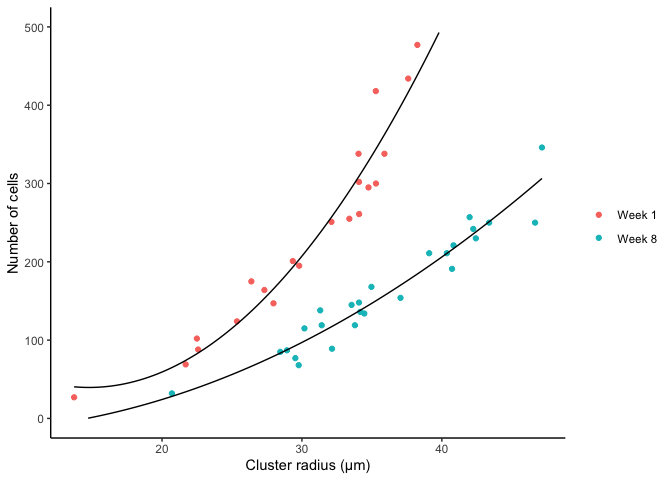
\includegraphics{Assignment2_forpdf_files/figure-latex/unnamed-chunk-17-1.pdf}

Visually, these functions seem to fit the data best! As I explained in
the intro for this section, when a cluster is very small, the addition
of a single cells or a small number of cells can have a big impact on
cluster size. But when a cluster is large, new cells are more
concentrated in the interior of the cluster, becoming more tightly
packed, and not contributing as much to cluster size. Since cells are
becoming more elongate over the course of the evolution experiment, they
can pack more easily, feel less internal stress, and don't reach a
growth block as quickly as the clusters from week 1.

\section{Conclusions}\label{conclusions}

Let's look at all the models side-by-side for easy comparison. I am
doing this with the plot\_grid() function from the ``cowplot'' package.

\begin{Shaded}
\begin{Highlighting}[]
\KeywordTok{plot_grid}\NormalTok{(plot1, plot2, plot3, plot4, }\DataTypeTok{labels =} \KeywordTok{c}\NormalTok{(}\StringTok{"mod1"}\NormalTok{, }\StringTok{"mod2"}\NormalTok{, }\StringTok{"mod3"}\NormalTok{, }\StringTok{"mod4"}\NormalTok{), }\DataTypeTok{hjust =} \OperatorTok{-}\FloatTok{1.3}\NormalTok{)}
\end{Highlighting}
\end{Shaded}

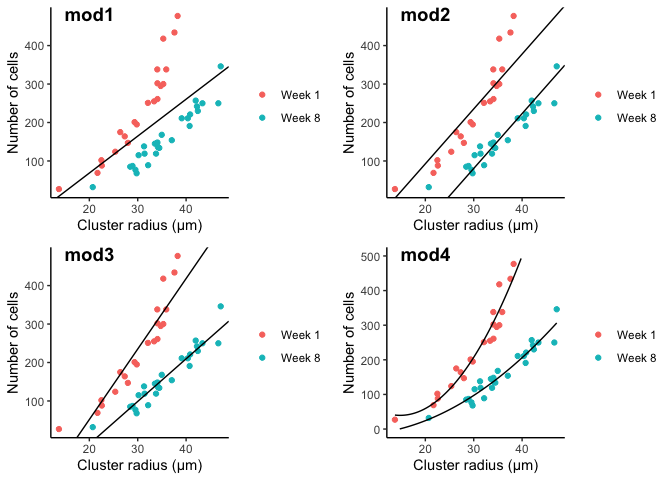
\includegraphics{Assignment2_forpdf_files/figure-latex/unnamed-chunk-18-1.pdf}

I chose to use a regular linear model for this data. A generalized
linear model would not apply because these are not count or binary data.
There are also no random effects because each data point represents an
individual from the same population, and different individuals are
measured at each time point. All the variables are accounted for, and
none of them produce a random effect.

Assumptions we make with a linear model are that we have equal variance
of residuals across the distribution, that the data are normally
distributed, and that the variables are independent.

We can use the plot function to view if the data meets these
assumptions. The first and third graphs of the output of the plot()
function for mod4 show that the residuals have equal variance because
the points are evenly distributed along the red line. The second graph
of the output shows that the data are normally distributed because the
points fall along the 1:1 line of the Q-Q plot. The 4th graph shows the
variables are independent because all the points fall within 0.5 Cook's
distance.

\begin{Shaded}
\begin{Highlighting}[]
\KeywordTok{plot}\NormalTok{(mod_}\DecValTok{4}\NormalTok{)}
\end{Highlighting}
\end{Shaded}

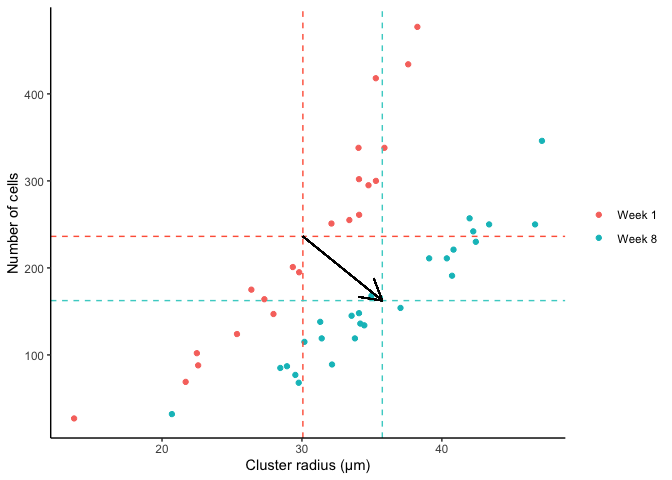
\includegraphics{Assignment2_forpdf_files/figure-latex/unnamed-chunk-19-1.pdf}
\includegraphics{Assignment2_forpdf_files/figure-latex/unnamed-chunk-19-2.pdf}
\includegraphics{Assignment2_forpdf_files/figure-latex/unnamed-chunk-19-3.pdf}
\includegraphics{Assignment2_forpdf_files/figure-latex/unnamed-chunk-19-4.pdf}

\begin{center}\rule{0.5\linewidth}{\linethickness}\end{center}

\subsection{Overall conclusions}\label{overall-conclusions}

Internal mechanical stress is a physical challenge for growing large
size in clonal cellular clusters. The evolution of snowflake yeast size
has been experimentally manipulated by imposing daily selection for
large size. Over time, snowflake yeast have been able to overcome
certain physical challenges to prevent cluster fracture while
maintaining large cluster size. They do so by increasing cell size
within the cluster as well as making cells more elongate to reduce
internal stress.

When we observe the characteristics of clusters from early and later in
the evolution experiment we notice several patterns. By week 8 of the
experiment clusters have gotten significantly larger, which we proved by
showing that mod2 was significantly different from mod1. Additionally,
week 8 clusters require fewer cells to grow the same amount as a week 1
cluster because each cell adds significantly more volume. We showed this
by testing mod3 against mod 2. Finally, because cells are becoming more
elongate over time, the internal stress is reduced and the week 8
clusters can continue to add more cells and grow even larger without
being constrained to a certain size like the week 1 clusters.

Here is a graph with the mean number of cells and cluster size marked
with a dashed line for each group (time point). This clearly
demonstrates that although cluster size is increasing, number of cells
per cluster is decreasing, and we can attribute this to the adaptations
of larger and more elongate cells.

\begin{Shaded}
\begin{Highlighting}[]
\NormalTok{week1 <-}\StringTok{ }\NormalTok{snowflake }\OperatorTok\StringTok{ }
\StringTok{  }\KeywordTok{filter}\NormalTok{(week }\OperatorTok{==}\StringTok{ "Week 1"}\NormalTok{)}
\NormalTok{week8 <-}\StringTok{ }\NormalTok{snowflake }\OperatorTok\StringTok{ }
\StringTok{  }\KeywordTok{filter}\NormalTok{(week }\OperatorTok{==}\StringTok{ "Week 8"}\NormalTok{)}

\NormalTok{plot }\OperatorTok{+}
\StringTok{  }\KeywordTok{geom_vline}\NormalTok{(}\DataTypeTok{xintercept =} \KeywordTok{mean}\NormalTok{(week1}\OperatorTok{$}\NormalTok{radius), }\DataTypeTok{linetype=}\StringTok{"dashed"}\NormalTok{, }\DataTypeTok{color =} \StringTok{"tomato"}\NormalTok{) }\OperatorTok{+}
\StringTok{  }\KeywordTok{geom_vline}\NormalTok{(}\DataTypeTok{xintercept =} \KeywordTok{mean}\NormalTok{(week8}\OperatorTok{$}\NormalTok{radius), }\DataTypeTok{linetype=}\StringTok{"dashed"}\NormalTok{, }\DataTypeTok{color =} \StringTok{"mediumturquoise"}\NormalTok{) }\OperatorTok{+}
\StringTok{  }\KeywordTok{geom_hline}\NormalTok{(}\DataTypeTok{yintercept =} \KeywordTok{mean}\NormalTok{(week1}\OperatorTok{$}\NormalTok{no_cells), }\DataTypeTok{linetype=}\StringTok{"dashed"}\NormalTok{, }\DataTypeTok{color =} \StringTok{"tomato"}\NormalTok{) }\OperatorTok{+}
\StringTok{  }\KeywordTok{geom_hline}\NormalTok{(}\DataTypeTok{yintercept =} \KeywordTok{mean}\NormalTok{(week8}\OperatorTok{$}\NormalTok{no_cells), }\DataTypeTok{linetype=}\StringTok{"dashed"}\NormalTok{, }\DataTypeTok{color =} \StringTok{"mediumturquoise"}\NormalTok{) }\OperatorTok{+}
\StringTok{  }\KeywordTok{geom_segment}\NormalTok{(}\KeywordTok{aes}\NormalTok{(}\DataTypeTok{x =} \KeywordTok{mean}\NormalTok{(week1}\OperatorTok{$}\NormalTok{radius), }\DataTypeTok{y =} \KeywordTok{mean}\NormalTok{(week1}\OperatorTok{$}\NormalTok{no_cells), }
                   \DataTypeTok{xend =} \KeywordTok{mean}\NormalTok{(week8}\OperatorTok{$}\NormalTok{radius), }\DataTypeTok{yend =} \KeywordTok{mean}\NormalTok{(week8}\OperatorTok{$}\NormalTok{no_cells)), }
                   \DataTypeTok{arrow =} \KeywordTok{arrow}\NormalTok{())}
\end{Highlighting}
\end{Shaded}

\begin{verbatim}
## Warning in grid.Call(C_textBounds, as.graphicsAnnot(x$label), x$x,
## x$y, : conversion failure on 'Cluster radius (μm)' in 'mbcsToSbcs': dot
## substituted for <ce>
\end{verbatim}

\begin{verbatim}
## Warning in grid.Call(C_textBounds, as.graphicsAnnot(x$label), x$x,
## x$y, : conversion failure on 'Cluster radius (μm)' in 'mbcsToSbcs': dot
## substituted for <bc>
\end{verbatim}

\begin{verbatim}
## Warning in grid.Call(C_textBounds, as.graphicsAnnot(x$label), x$x,
## x$y, : conversion failure on 'Cluster radius (μm)' in 'mbcsToSbcs': dot
## substituted for <ce>
\end{verbatim}

\begin{verbatim}
## Warning in grid.Call(C_textBounds, as.graphicsAnnot(x$label), x$x,
## x$y, : conversion failure on 'Cluster radius (μm)' in 'mbcsToSbcs': dot
## substituted for <bc>
\end{verbatim}

\begin{verbatim}
## Warning in grid.Call(C_textBounds, as.graphicsAnnot(x$label), x$x,
## x$y, : conversion failure on 'Cluster radius (μm)' in 'mbcsToSbcs': dot
## substituted for <ce>
\end{verbatim}

\begin{verbatim}
## Warning in grid.Call(C_textBounds, as.graphicsAnnot(x$label), x$x,
## x$y, : conversion failure on 'Cluster radius (μm)' in 'mbcsToSbcs': dot
## substituted for <bc>
\end{verbatim}

\begin{verbatim}
## Warning in grid.Call(C_textBounds, as.graphicsAnnot(x$label), x$x,
## x$y, : conversion failure on 'Cluster radius (μm)' in 'mbcsToSbcs': dot
## substituted for <ce>
\end{verbatim}

\begin{verbatim}
## Warning in grid.Call(C_textBounds, as.graphicsAnnot(x$label), x$x,
## x$y, : conversion failure on 'Cluster radius (μm)' in 'mbcsToSbcs': dot
## substituted for <bc>
\end{verbatim}

\begin{verbatim}
## Warning in grid.Call(C_textBounds, as.graphicsAnnot(x$label), x$x,
## x$y, : conversion failure on 'Cluster radius (μm)' in 'mbcsToSbcs': dot
## substituted for <ce>
\end{verbatim}

\begin{verbatim}
## Warning in grid.Call(C_textBounds, as.graphicsAnnot(x$label), x$x,
## x$y, : conversion failure on 'Cluster radius (μm)' in 'mbcsToSbcs': dot
## substituted for <bc>
\end{verbatim}

\begin{verbatim}
## Warning in grid.Call(C_textBounds, as.graphicsAnnot(x$label), x$x,
## x$y, : conversion failure on 'Cluster radius (μm)' in 'mbcsToSbcs': dot
## substituted for <ce>
\end{verbatim}

\begin{verbatim}
## Warning in grid.Call(C_textBounds, as.graphicsAnnot(x$label), x$x,
## x$y, : conversion failure on 'Cluster radius (μm)' in 'mbcsToSbcs': dot
## substituted for <bc>
\end{verbatim}

\begin{verbatim}
## Warning in grid.Call(C_textBounds, as.graphicsAnnot(x$label), x$x,
## x$y, : conversion failure on 'Cluster radius (μm)' in 'mbcsToSbcs': dot
## substituted for <ce>
\end{verbatim}

\begin{verbatim}
## Warning in grid.Call(C_textBounds, as.graphicsAnnot(x$label), x$x,
## x$y, : conversion failure on 'Cluster radius (μm)' in 'mbcsToSbcs': dot
## substituted for <bc>
\end{verbatim}

\begin{verbatim}
## Warning in grid.Call.graphics(C_text, as.graphicsAnnot(x$label), x$x,
## x$y, : conversion failure on 'Cluster radius (μm)' in 'mbcsToSbcs': dot
## substituted for <ce>
\end{verbatim}

\begin{verbatim}
## Warning in grid.Call.graphics(C_text, as.graphicsAnnot(x$label), x$x,
## x$y, : conversion failure on 'Cluster radius (μm)' in 'mbcsToSbcs': dot
## substituted for <bc>
\end{verbatim}

\includegraphics{Assignment2_forpdf_files/figure-latex/unnamed-chunk-20-1.pdf}

\begin{center}\rule{0.5\linewidth}{\linethickness}\end{center}

I made four progressively more complex models, and the last, most
complex one turned out to be the best according to the p-values. Higher
complexity doesn't always mean a better model according the Akaike
Information Criterion, which penalizes model complexity in balance with
rewarding good model fit. Just for fun I'll perform some data dredging
using the dredge() function from the ``MuMIn'' package. It will give us
the AIC for each possible model within the parameter space I set.

\begin{Shaded}
\begin{Highlighting}[]
\NormalTok{full <-}\StringTok{ }\KeywordTok{lm}\NormalTok{(no_cells }\OperatorTok{~}\NormalTok{(.)}\OperatorTok{^}\DecValTok{2}\NormalTok{, }\DataTypeTok{data =}\NormalTok{ snowflake, }\DataTypeTok{na.action =}\NormalTok{ na.fail)}
\NormalTok{dredge <-}\StringTok{ }\KeywordTok{dredge}\NormalTok{(full, }\DataTypeTok{rank =} \StringTok{"AICc"}\NormalTok{)}
\end{Highlighting}
\end{Shaded}

\begin{verbatim}
## Fixed term is "(Intercept)"
\end{verbatim}

\begin{Shaded}
\begin{Highlighting}[]
\NormalTok{dredge}
\end{Highlighting}
\end{Shaded}

\begin{verbatim}
## Global model call: lm(formula = no_cells ~ (.)^2, data = snowflake, na.action = na.fail)
## ---
## Model selection table 
##    (Int)    rds wek rds:wek df   logLik  AICc delta weight
## 8 -314.6 18.320   +       +  5 -231.660 474.8  0.00  0.999
## 4 -192.7 14.260   +          4 -240.304 489.6 14.78  0.001
## 2 -123.4  9.599              3 -273.098 552.8 77.97  0.000
## 3  236.2          +          3 -281.846 570.3 95.47  0.000
## 1  195.4                     2 -284.972 574.2 99.43  0.000
## Models ranked by AICc(x)
\end{verbatim}

In fact, the model with the most estimated terms (df = 5) has the lowest
AIC and highest weight. Our analysis is supported!


\end{document}
